\documentclass[11pt]{article}
\usepackage[top=1in, bottom=1in, left=1in, right=1in]{geometry}
\usepackage{physics}

\usepackage{listings}
\lstset{frame = tb, language = Python,
		aboveskip = 3mm, belowskip = 3mm,
		tabsize = 3, columns = flexible,
		basicstyle = \small\ttfamily}

\usepackage{graphicx}
\graphicspath{{c:/Users/Jacob/Documents/Coding_Stuff/LaTeX/Honors_Thesis/Figures/}}

\usepackage{fancyhdr}
\pagestyle{fancy}
\renewcommand{\sectionmark}[1]{\markboth{#1}{}}

\fancyhf{}
\fancyhead[R]{\leftmark}
\fancyhead[L]{Monte Carlo and Lattice QCD}
\fancyfoot[C]{\thepage}
\fancypagestyle{plain}{\fancyhf{}
	\renewcommand{\headrulewidth}{0pt}}

\usepackage{tikz}
\usetikzlibrary{shapes.callouts}
\tikzset
{
	line/.style = {black},
	transition/.style = {dashed, black}
}

\begin{document}
\section{The Ising Model}
The Ising model is a good place to begin with the Metropolis algorithm because of its simplicity. On the lattice for the Ising model, the interaction is nearest-neighbor and discrete. For each lattice site $k$, there is a corresponding spin $s_k\in\{-1,1\}$. Given this, the Hamiltonian for the Ising model is
\begin{align}
	H=-\sum_{\langle i,j\rangle}J_{i,j}s_is_j+h\sum_js_j
\end{align}
where $J_{i,j}$ is the interaction strength between neighbors at site $i$ and site $j$ and $h$ is an external magnetic field. If we assume no external magnetic field and a constant interaction strength, then we obtain
\begin{align}
	H=-J\sum_{\langle i,j\rangle}s_is_j.
	\label{eq:Energy}
\end{align} Since each site has two possibilities, for a $d$-dimensional hypercube with side length $n$, there are $2^{n^d}$ possibilities for the lattice. This is the advantage of using Monte Carlo techniques. Many measurements of the lattice can be made to simulate the model and derive an accurate evolution on which observables can be measured. In the case for the Ising model, and subsequent models, the Metropolis algorithm is used.

\subsection{Application of the Metropolis Algorithm}

For the evolution of the Ising model, one must decide whether a change in the lattice should occur or not. The Metropolis algorithm gives the probability $P(\vb{x}_{\ell+1}\mid \vb{x}_\ell)$ for a transition from state $x_\ell$ to $x_{\ell+1}$. If the change in energy $\Delta H$ is less than zero, then the change at the site will occur since the system tends towards a lowest energy state. Otherwise, the transition probability follows the Boltzmann distribution $e^{-\beta\Delta H}$ where $\beta=1/k_BT$. Thus, the Metropolis transition probability is
\begin{align}
	P(\vb{x}_{\ell+1}\mid \vb{x}_\ell)=
	\begin{cases}
		e^{-\beta\Delta H},\quad&\text{if }\Delta H>0\\
		1,&\text{otherwise.}
	\end{cases}
	\label{eq:ProbIsing}
\end{align}
To obtain the change in energy $\Delta H$, a new state must be chosen for the lattice site. In the case of the Ising model, there are only two states: $\pm1$. Therefore, the new energy is just the opposite sign of the old energy according to equation \ref{eq:Energy}. Thus, the change in energy at lattice site $j$ is double the original energy at that site, or
\begin{align}
	\Delta H_j=-2Js_j\sum_is_i.
	\label{eq:DeltaH}
\end{align}
So the change in energy can be calculated this way since the new spin being chosen for site $j$ is implicit in the equation. For later simulations, this is not the case and so a slightly different state is chosen randomly to calculate the change induced by the new state. Now to apply this, the steps for the evolution of the Ising model are as follows:
\begin{enumerate}
\item Choose a lattice site $j$.
\item Calculate the change in energy $\Delta H_j$ at the site $j$.
\item If $\Delta H<0$ then change the spin at site $j$.
\item Otherwise assign it a probability $\exp(-\beta\Delta H_j)$ of changing.
\item Repeat steps 1-4 for every site on the lattice.
\end{enumerate}

This completes one sweep of the lattice as every site on the lattice is checked to flip. Step 4 can be completed by randomly choosing a number $a\in[0,1]$ such that if $a<\exp(-\beta\Delta H)$ the change occurs otherwise the change is rejected.

A problem faced by virtue of a finite lattice is the boundary. In this model, the boundary lattice sites are missing neighbors due to the limitations of a computer simulation. One solution to this problem, which is used in the simulations in this paper, is periodic boundary conditions. The missing neighbors of the boundary sites are replaced by the sites on the opposite side of the lattice.

\begin{figure}[ht]
\centering
\begin{tikzpicture}
	\draw[gray, thick,] (0,2) -- (0,-2);
	\draw[gray, thick] (2,0) -- (-2,0);
	\filldraw[black] (0,0) circle (1.5pt);
	\node[above] at (0,2) {\footnotesize($x$, $(y+1)\text{mod}N$)};
	\node[right] at (2,0) {\footnotesize($(x+1)\text{mod}N$, $y$)};
	\node[below] at (0,-2) {\footnotesize($x$, $(y-1)\text{mod}N$)};
	\node[left] at (-2,0) {\footnotesize($(x-1)\text{mod}N$, $y$)};
	\node[below right] at (0,0){\footnotesize($x$, $y$)};
\end{tikzpicture}
\caption{Neighboring sites of site $(x,y)$ with periodic boundary conditions} \label{fig:PBC}
\end{figure}

For example, on a square 2-dimensional lattice with sides $N$, the neighbors of any site $(x,y)$ will be as shown in figure \ref{fig:PBC} where mod represents the modulo operator. As long as the interactions are shorter than the lattice size, then the lattice is effectively infinite for each point. The interactions for the Ising model are nearest-neighbor, so periodic boundary conditions are applied for the boundary sites.

\subsection{Measurements on the Lattice}
\subsubsection{Magnetization}
Now with the ability to model the Ising Model, measurements can now be made. It is helpful to note that dimensionality has so far been arbitrary with exception to the remarks on figure \ref{fig:PBC}. For $d$ dimensions, for each lattice site $(x_1,x_2,\ldots,x_d)$, it would have $2d$ neighbors for measurement of the change in energy. One measurement is magnetization given by
\begin{align}
	M=\sum^{N^2}_{j=1}s_j
\end{align}
and the magnetization per spin is just $m=M/L^2$. What should be expected for the magnetization of this system?

From equation \ref{eq:ProbIsing}, one can see there are just two parameters: the temperature $T$ and the interaction strength $J$. But these can just be written as one parameter $T_J=J/k_BT_c$ (with the Boltzmann constant included) since they have the same effect on $\Delta H$. At some point, the system will reach an equilibrium where $m$ will oscillate about some value. Because $T_J>0$, the interactions are ferromagnetic and so spins will tend to align in the same direction. This is seen at low $T$ since the thermal energy is not large enough to overcome the alignment. Therefore, the lattice will be highly ordered with $\abs{m}\approx1$ or slightly less. But with high $T$, the magnetic interactions will be dominated by the thermal energy and neighboring spins will not be correlated; so $m\approx0$. There is some temperature at which the thermal energy is larger than the magnetic interactions of the lattice sites. This is the critical temperature $T_c$.
\begin{figure}[ht]
\begin{lstlisting}
def Ising2D(lattice, Jkbt, N):
    magnetization = 0

    for p in product(range(N), range(N)):
        i, j = p
        energy = (lattice[i][(j - 1) % N] + lattice[i][(j + 1) % N] +
                   lattice[(i - 1) % N][j] + lattice[(i + 1) % N][j]) *
                   lattice[i][j]
        magnetization += lattice[i][j]

        if energy <= 0 or np.random.random() < np.exp(-2 * Jkbt * energy):
            lattice[i][j] *= -1

    return lattice, magnetization
\end{lstlisting}
    \caption{Python code for one sweep of a $N$x$N$ lattice with $T_J=\texttt{Jkbt}$. The change in energy, $\Delta H$, for a site is calculated and stored in \texttt{energy} where then a Metropolis update is performed. Also, the magnetization at that site is stored in \texttt{magnetization} and is used later to determine the equilibrium magnetization of the lattice. This is carried out for every site on the lattice, then returning the updated lattice and its total magnetization.} \label{fig:Ising2DCode}
\end{figure}

In figure \ref{fig:Ising2DCode}, the function that completes one sweep of the lattice is shown. Each lattice site is checked to change before the next site is checked. The \texttt{product} function in the for loop creates tuples whose values are stored in \texttt{i} and \texttt{j} for each loop thus completing the sweep row by row. If the energy change is accepted according to the if statement, the spin value at the lattice site is flipped. It is important to note that the lattice must be thermalized before measurements can be taken, that is the lattice must first reach an equilibrium. This is done by completing enough lattice sweeps before taking measurements. The Ising model simulations discussed are done with 10000 sweeps and only the latter fourth of sweeps are measured. The application of this function is shown in its entirety in the appendix. 

For the parameter $T_J$, the critical temperature is at $T_J=\frac{1}{2}\ln(1+\sqrt{2})$. In figure \ref{fig:MvTdN}, the behavior of different temperatures on different lattice sizes is shown. The absolute magnetization is measured instead of the signed magnetization because the magnetization at which a specific lattice settles to can be either $\pm x$ for $x\in[0,1]$ and the magnetization can rarely but suddenly switch signs due to finite size of the lattice. Ignoring the sign fixes these issues and the result is shown in figure \ref{fig:MvTdN}; for low $T$, the lattice is more ordered and the absolute magnetization is near 1. For high $T$, the magnetization oscillates about 0 as discussed above. Since the absolute value of the magnetization is measured, the values plotted for high temperature represent the magnitude of these oscillations. For the smaller lattice size (e.g. $N=5$), the oscillations will be larger since each site will have a greater impact on the total magnetization of the lattice.

\begin{figure}[h]
	\centering
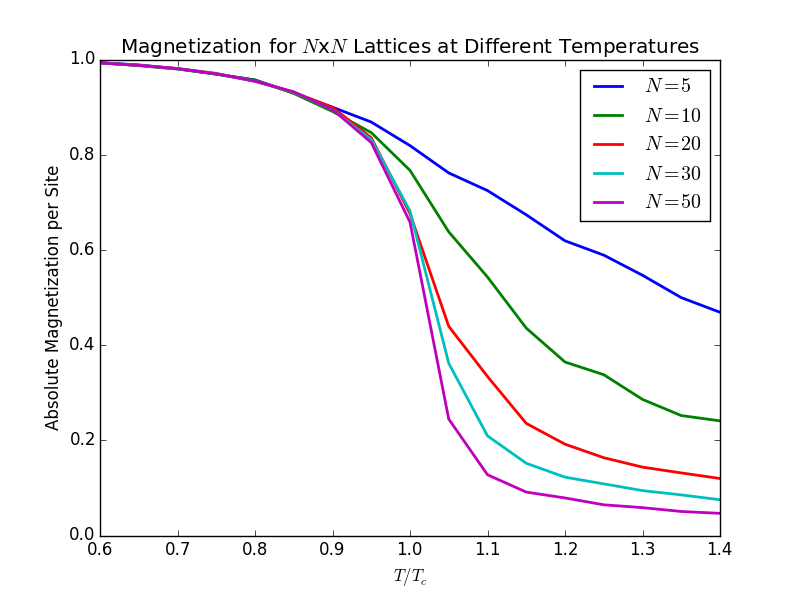
\includegraphics[scale=0.60]{Mag_vs_T_Different_N.png}
	\caption{The normalized magnetization plotted against temperature with respect to the critical temperature for various lattice sizes. The values were computed by evolving the lattice until equilibrium, then computing the average for many measurements of the magnetization.}
	\label{fig:MvTdN}
\end{figure}

\subsubsection{Susceptibility}

Susceptibility can also be measured on the lattice. It is the measure of the change in magnetization due to a magnetic field. The effect of lattice size and temperature on magnetic susceptibility $\chi$ can also be measured by
\begin{align}
	\chi&=\pdv{\langle M\rangle}{H}\\
	&=\frac{1}{T}(\langle M^2\rangle-\langle \abs{M}\rangle^2).
	\label{eq:Sus}
\end{align}
This measurement only requires the average magnetization, which is already measured, and the average of the squared magnetization. In the simulation for figure \ref{fig:MvTdN}, the susceptibility was also measured using equation \ref{eq:Sus} as shown in figure \ref{fig:SvTdN}. A large susceptibility occurs where there is a large standard deviation in the magnetization of the sweeps (the susceptibility is the variance of the magnetization). At low $T$, the lattice is in equilibrium at some magnetization and at high $T$, the lattice is unordered and so the magnetization does not vary far from 0. In either case, the variance is small. At $T=T_c$, the lattice does not reach an equilibrium and so the change in magnetization is large accounting for the large peak in figure \ref{fig:SvTdN}.

\begin{figure}[h]
	\centering
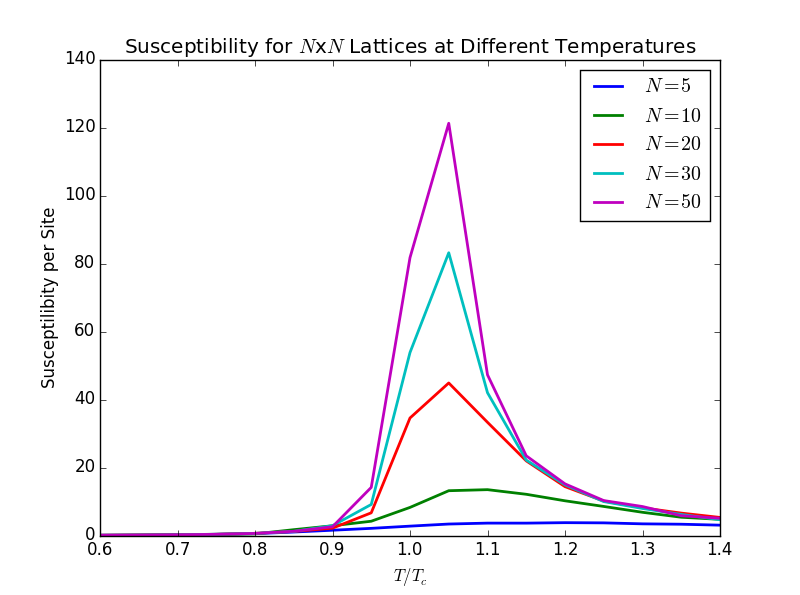
\includegraphics[scale=0.60]{Sus_vs_T_Different_N.png}
	\caption{The normalized susceptibility for the same simulation as figure \ref{fig:MvTdN}.}
	\label{fig:SvTdN}
\end{figure}

The Metropolis algorithm allowed us to model an Ising model system. With a model, measurements can be made on the system; the measurement of magnetization dependent on the parameters of the system was done above. Other measurements such as specific heat or correlation length can be made. Also, a variable interaction strength, nonzero external magnetic field or a higher dimensional model can have significant changes on the system with little change to the program. Going forward, the Monte Carlo method and the steps of the Metropolis algorithm used here will be applied for more complicated systems, specifically with respect to the discretized version of the Feynman path integral.
\end{document}